\graphicspath{{chapt_dutch/}{intro/}{chapt2/}{chapt3/}{chapt4/}{chapt5/}{chapt6/}{chapt7/}{chapt8/}}

% Header
\renewcommand\evenpagerightmark{{\scshape\small Chapter 7}}
\renewcommand\oddpageleftmark{{\scshape\small Corrections to simulation}}

\hyphenation{}

\chapter[Corrections to simulation and systematic uncertainties]%
{Corrections to simulation}
\label{chapt:8}
\section{Corrections to simulation}\label{sec:correc_sim}
\subsection{Pile-up re-weighting}
\label{sec:pileup}

\subsection{Jet Energy Scale}
\label{sec:jes}

\subsection{Jet Energy Resolution}
\label{sec:jer}

\subsection{B tagging}
\label{sec:btag}

\subsection{Trigger, Lepton ID and Isolation}
\label{sec:trig_lepIdIso}

\subsection{Generator level weights}
\label{sec:genweights}

\subsection{Top quark $p_{T}$}
\label{sec:topPt_correc}

\begin{figure}[htp]
\centering
\begin{tabular}{cc}
\hspace{-0.5cm}
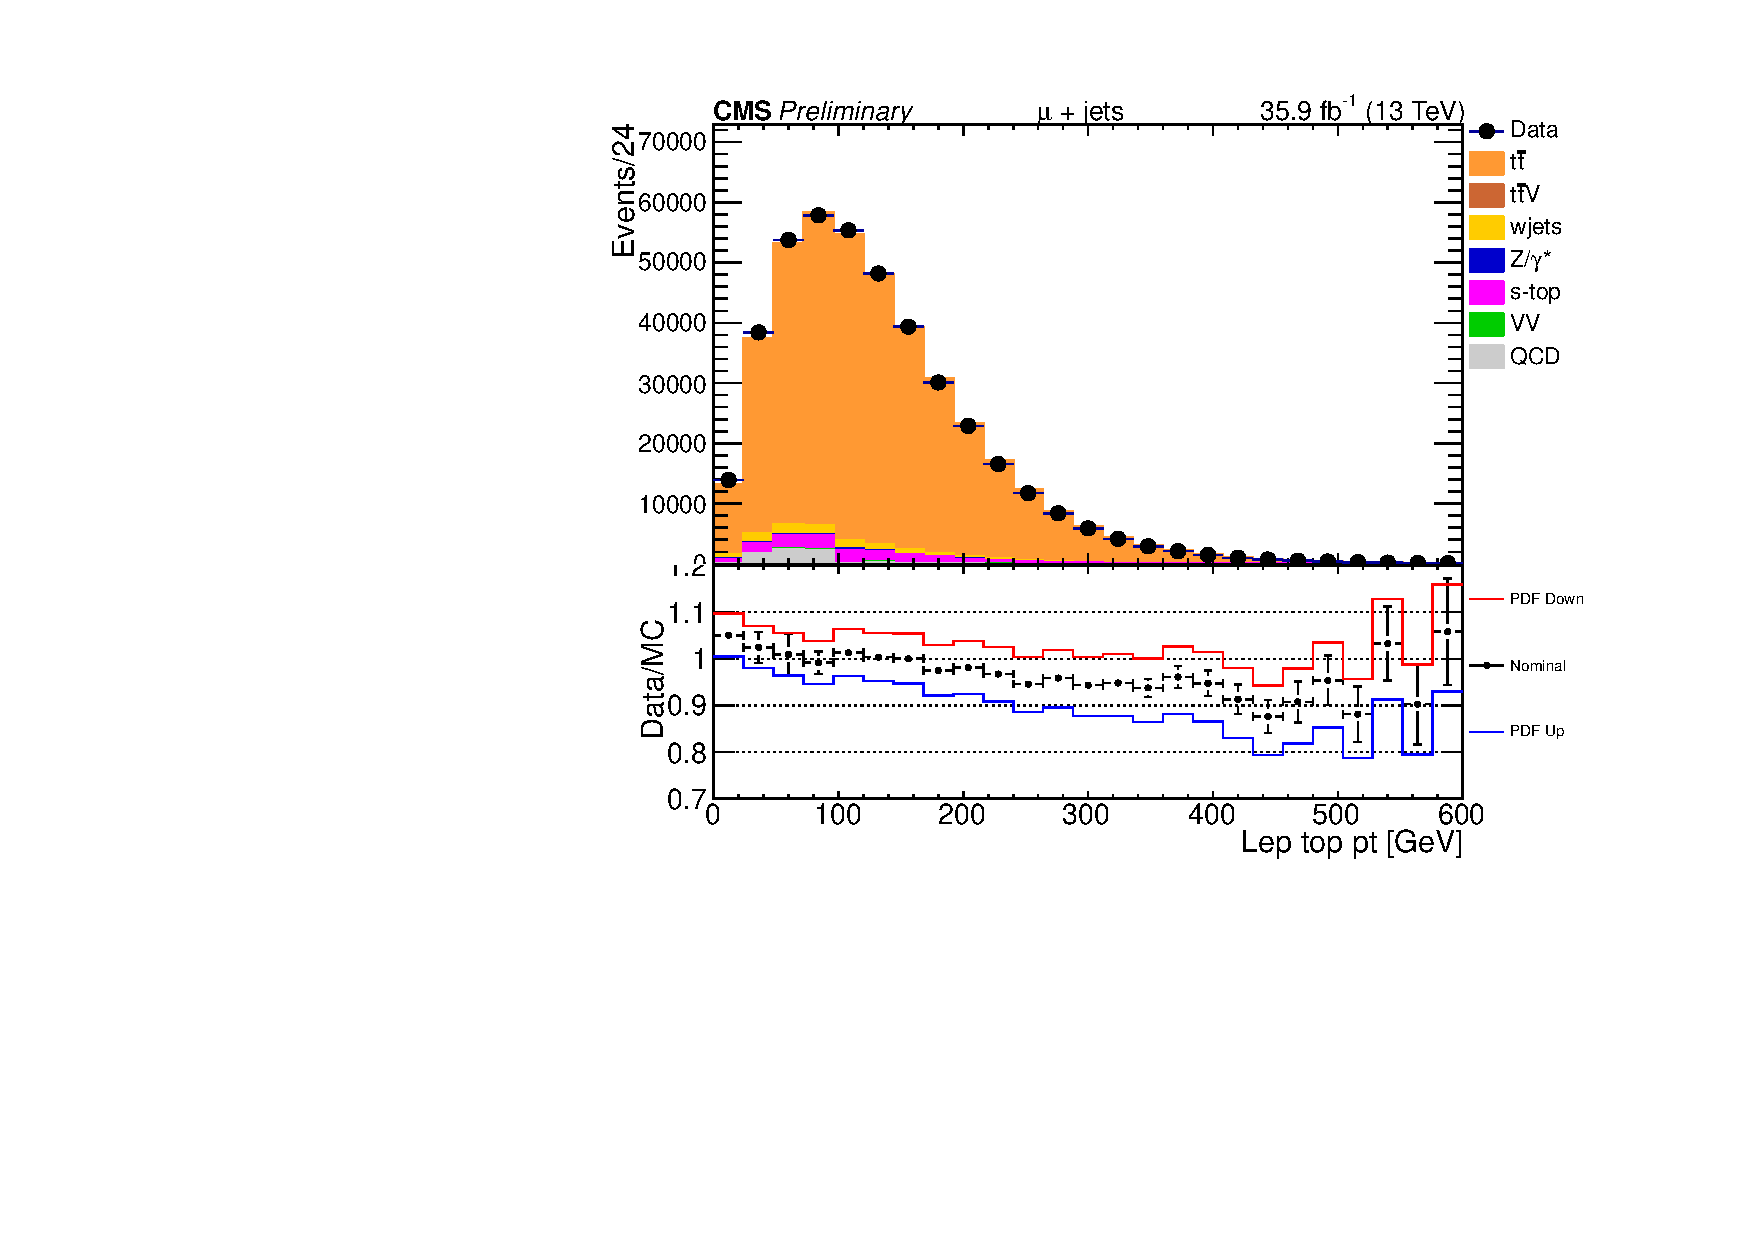
\includegraphics[scale=0.45]{fig/correc_uncer/lep_topPT_pdf.pdf}
& \hspace{-1.50cm} 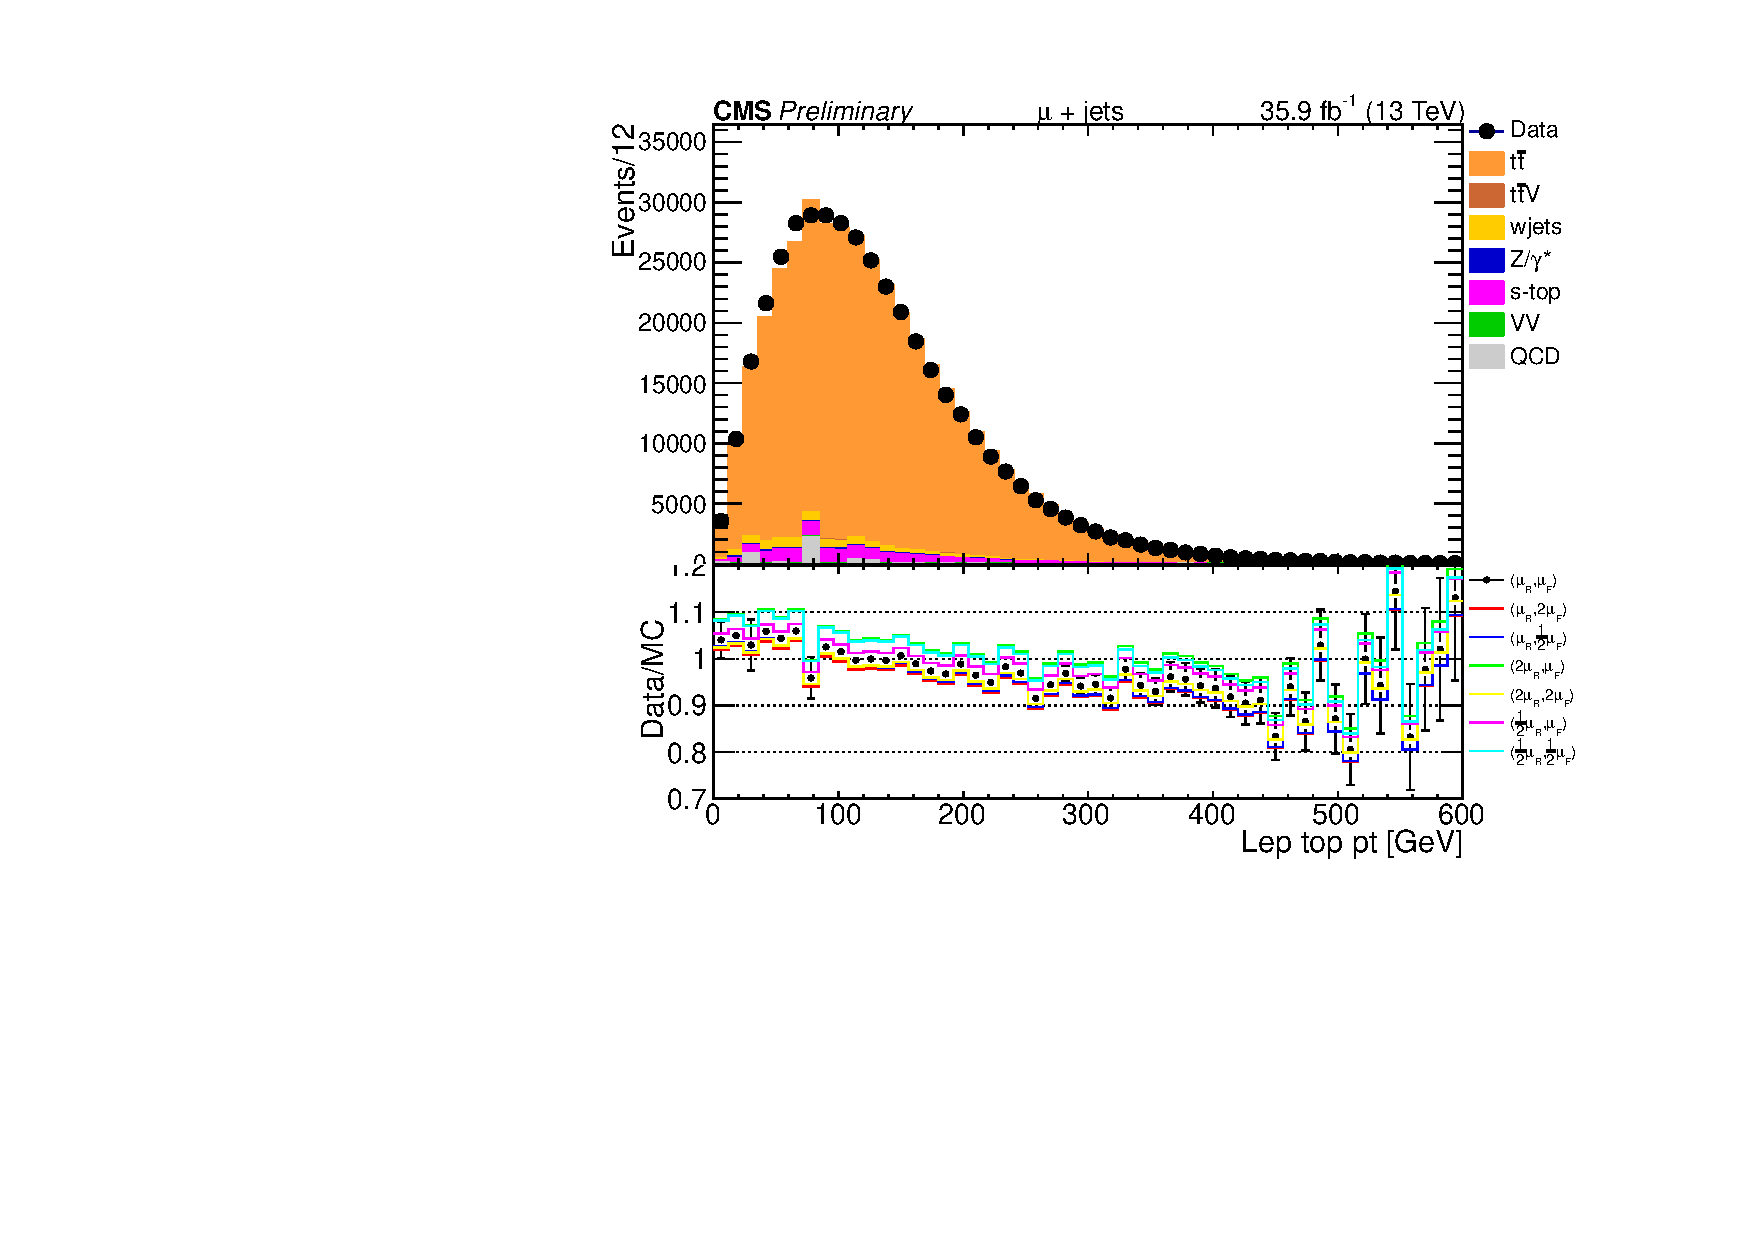
\includegraphics[scale=0.45]{fig/correc_uncer/lep_top_ren_fac.pdf}\\
  \qquad ($\mathbf{a}$)\qquad\qquad&($\mathbf{b}$)\qquad\qquad\qquad\qquad \\
\end{tabular}
\caption{ }\label{fig:top_pt_correc_expec}
\end{figure}

\section{Systematic uncertainties}\label{sec:sys_unc}
\subsection{Luminosity}
\label{sec:syslumi}

\subsection{Pileup}
\label{sec:syspileup}

\subsection{Jet energy scale}
\label{sec:sysjes}

\subsection{Jet energy resolution}
\label{sec:sysjer}

\subsection{Unclustered MET}
\label{sec:sysmet}

\subsection{b-tagging and misidentification efficiencies}
\label{sec:sysbtag}

\subsection{Lepton trigger/isolation/identification efficiencies}
\label{sec:systrigg}


%\renewcommand*{\thesection}{\thechapter.\arabic{section}}       % reset again to chaptnum.sectnum

\clearpage{\pagestyle{empty}\cleardoublepage}
